\section{Assessment of computational reproducibility}

\subsection{Set-up}

\subsubsection{Create repository using template}
\timeno

Use the STARS computational reproducibility template to create a new repository.

\begin{itemize}
    \item Template: \url{https://github.com/pythonhealthdatascience/stars_reproduction_template}. To use it, select the "Use this template" button.
    \item Organisation: \url{https://github.com/pythonhealthdatascience}
    \item Repository name: stars-reproduce-firstauthorsurname-publicationyear
    \item Description: Assessing the computational reproducibility of [firstauthor et al. publicationyear] as part of STARS.
    \item Public repository
\end{itemize}

\subsubsection{Upload journal article and all artefacts to the repository}
\timeno

Upload all available materials from the article to the repository. This could include:
\begin{itemize}
    \item Journal article
    \item Supplementary materials
    \item Code (for example, copying the content of a GitHub repository)
    \item Protocol
\end{itemize}

\hl{Add more information on locations (i.e. this is all in one seperate location that don't touch - but work on it and add eg the tables and figures, into another location)}

\subsubsection{Select license}
\timeno

Select a license for the repository. At this stage, this should be as permissive as possible, whilst being compatible with the license used by the study authors. For instructions on how to add a license to a repository, see \url{https://docs.github.com/en/communities/setting-up-your-project-for-healthy-contributions/adding-a-license-to-a-repository}.

\subsection{Scope of reproduction}

\subsubsection{Read the journal article}
\timeyes

Read through the journal article and supplementary materials (but not yet looking into the code or data). Consolidate this by adding a short description of the article to the Quarto book. This should be relatively concise, and cover the key methods and results. It might, for example, include any model flow diagram provided in the paper, any model parameters mentioned, and the model type and software. This can also be updated later.

\subsubsection{Make consensus decision on scope}
\timeyes[for scoping (not discussion)]

The next step is to define the scope of the reproducibility study - in other words, what parts of the paper you intend to reproduce. The scope should include:
\begin{enumerate}[label=(\alph*)]
    \item All tables and figures within the manuscript that contain results from the simulation, and-
    \item Any other key results in the paper, that are not otherwise captured within the tables and figures. "Key results" can be considered things that are mentioned within the abstract or conclusion, or feature prominently within the results section.
\end{enumerate}

This does not need to include tables and figures in the Appendices (unless these are identified as "key results"). This method of defining the scope is based on that used by Wood et al. 2018.\autocite{wood_replication_2018, wood_push_2018}

Whilst the rest of this protocol is conducted by a single member of the STARS team, the scope of the reproducibility study will be defined as a consensus decision, with at least two team members reading the article and suggesting the scope independently, and then agreeing together on what is appropriate.

\subsubsection{Compile items in scope}
\timeyes

Once the scope has been decided, upload each item to the repository.

\begin{itemize}
    \item For tables, download a CSV version of each if available. Otherwise, convert the tables into CSV format.
    \item For figures, download the highest-quality version of each figure that is available. Then extract data from the figures. \hl{Do we want to do this? Do we trust the software?} Software available: \url{https://plotdigitizer.com/best-plot-digitizer}. Good options are:
    \begin{itemize}
        \item WebPlotDigitizer (\url{https://automeris.io/posts/}) - in active development, version 4 and below are GNU AGPL v3, version 5 (published 14 May 2024) and onwards will be closed source.
        \item Enguage Digitizer (\url{https://markummitchell.github.io/engauge-digitizer/}) - no further development since 3 years ago, GNU GPL v2
    \end{itemize}
    \item For results described in the text (but not captured in a table or figure), record in a format appropriate to then later compare against (for example, within a CSV).
\end{itemize}

\subsubsection{Archive scope and supporting documents on Zenodo}
\timeyes

Describe the scope within the Quarto book, providing justification for any "key results" chosen, and including reference to the uploaded figures and data for the items. Any tables and figures not being produced (for example, as they don't contain results from the simulation) should also be noted.

With the organisation linked to Zenodo, toggle Zenodo to preserve that repository, and then create a release on GitHub, which Zenodo will then automatically download and register with a DOI. This release should serve as a public registration of the intended scope of the reproducibility study, and archiving the repository at this point (prior to having started using or really looking at the the code).

As stated in the "Guide for Accelerating Computational Reproducibility (ACRe) in the Social Sciences", it is important that the scope is defined at the start of the study, and publicly archived so as not to be amended during the course of the study.\cite{berkeley_initiative_for_transparency_in_the_social_sciences_guide_2022}

\subsection{Familiarise with artefacts}

\subsubsection{Describe code/data}
\timeyes

Browse through any code and any data that you uploaded to the repository. In the Quarto book, add a tree of the uploaded files, along with one-sentence description of each file.

This is as suggested by Ayllón et al. 2021\autocite{ayllon_keeping_2021} in their guidelines for keeping modelling notebooks

\subsubsection{Search for code that produces items in scope}
\timeyes

As in Krafczyk et al. 2021,\cite{krafczyk_learning_2021} look over the code and any data, and attempt to identify sections that correspond with items in the scope. Record this within the log.

\subsection{Set up environment}

\subsubsection{Identify dependencies}
\timeyes

To ensure a reproducible research environment, we need to know:
\begin{itemize}
    \item The operating system used (e.g. Windows, Mac, Linux) and its version 
    \item The software used (e.g. Python, R)
    \item The software packages used and their versions\autocite{the_turing_way_community_turing_2022}
\end{itemize}

However, it is likely that papers may not include all the information required (such as versions used). In which case:
\begin{itemize}
    \item No operating system - use Linux
    \item No operating system version - use closest to publication date \hl{Do we want to be this stringent?}
    \item No package list - look at the libraries/packages imported within the scripts
    \item No package versions - use closest to publication date
\end{itemize}

\subsubsection{Create environment}
\timeyes

\hl{Evaluate these options. Consider whether they control OS. Consider whether they control date. But also - whether we want that. How casual vs. standardised on this we want to be.}

One suggestion is to install packages and their dependencies at a point in time no later than publication date. Not all solutions below guarantee this though. The publication date is used as could have re-run code during approval process, but know not after publication.
\begin{itemize}
    \item Anecdotally, this could be particularly handy for R which often tries to get the most recent packages
\end{itemize}

Another suggestion is to match operating system to developer. Again, not all solutions below guarantee this. This will also be relevant later if want to test reproduction package on different operating systems.

Python -
\begin{itemize}
    \item Conda, VirtualEnv, etc.
    \item Docker - to do development inside container, VSCode Dev Containers extension allows you to open folder inside container - \href{https://code.visualstudio.com/docs/devcontainers/containers}{source 1}
\end{itemize}

R -
\begin{itemize}
    \item Renv
    \item Posit Public Package Manager - can use Snapshot (earliest is Oct 2017, and 5 most recent versions of R), for Linux can install binary packages (which is much quicker, as usually R installs from source rather than binary unlike for Windows and Mac which makes it really slow) - \href{https://packagemanager.posit.co/client/#/repos/cran/setup}{source 1}, \href{https://docs.posit.co/faq/p3m-faq/#frequently-asked-questions}{source 2}
    \item Groundhog - can go back to R 3.2 and April 2015 (and apparently can patch to go earlier) - \href{https://www.brodrigues.co/blog/2023-01-12-repro_r/}{source 1}
    \item miniCRAN - \href{https://learn.microsoft.com/en-us/sql/machine-learning/package-management/create-a-local-package-repository-using-minicran?view=sql-server-ver16}{source 1}
    \item Docker - requires license for non-academic (e.g. NHS) use - but Podman can drop in as replacement. To do development inside a container isn't natively supported by RStudio but can use RStudioServer via Rocker. By default, it runs in ephemeral mode - any code created or saved is lost when close - but you can use volume argument to mount local folders - \href{https://towardsdatascience.com/running-rstudio-inside-a-container-e9db5e809ff8}{source 1}
\end{itemize}

\subsubsection{Update license if necessary}

As above, we want to use a license that is as permissive as possible whilst being compatible with the license used by the author, as well as now the license of any packages used within the project. To identify the licenses used:
\begin{itemize}
    \item In Python, you could use the package "pip-licenses" (\url{https://pypi.org/project/pip-licenses/})
    \item In R, you can run the command \texttt{installed.packages(fields = "License")}
\end{itemize}

If it is not possible to use a completely permissive license like MIT, explain why (either due to author license or package licenses). An example for how this can be displayed is as follows \hl{Add appropriate citation https://github.com/TomMonks/stars-treat-simmer/tree/main/img}:

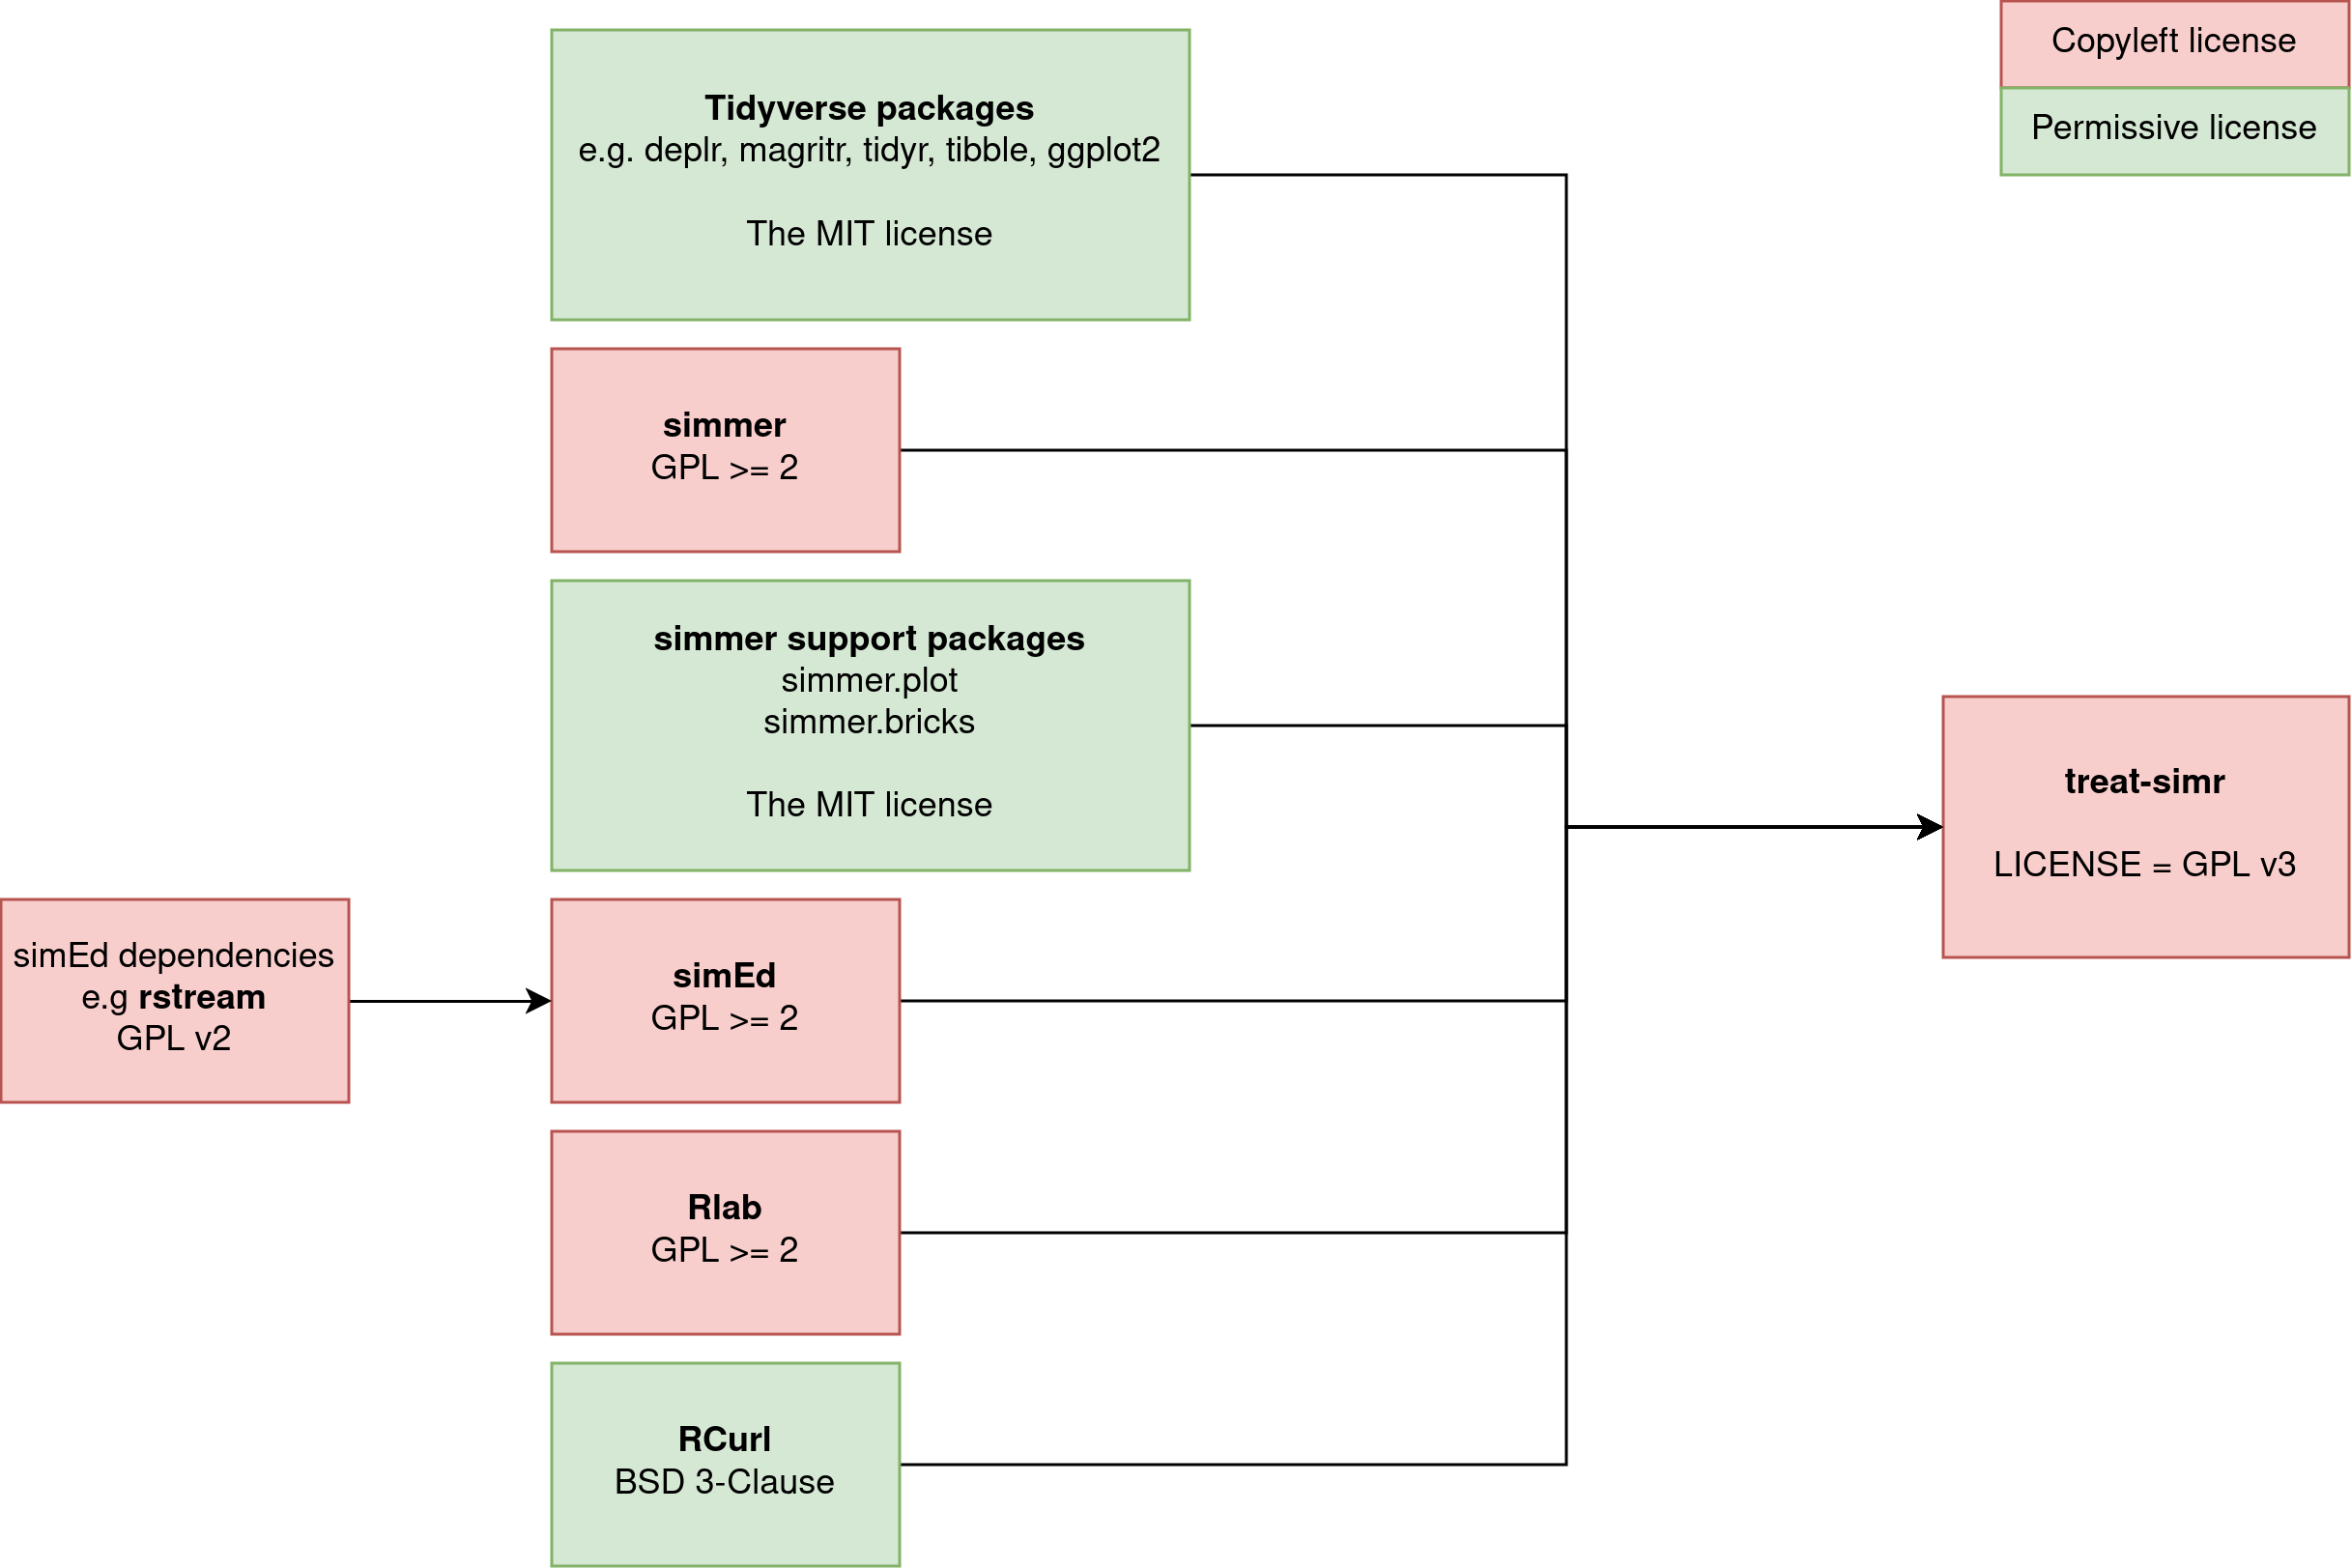
\includegraphics[width=\linewidth]{images/license.png}

\subsection{Attempt to reproduce items in scope}

\subsubsection{Use provided code to produce notebook creating items in scope}
\timeyes[(except long computation, at researcher discretion)]

Run the code and attempt to produce the items in the scope. Insert the code into a notebook (.ipynb or .Rmd) as this enables you to easily share the code and produced outputs from the scope. Label each output clearly, as it relates to the manuscript.

\hl{consider whether want makefile etc or not, can look at sources for reproduction package section, this might be simplest solution though}

Whilst running this code, the researcher should be troubleshooting issues and evaluating reproduction success, as below.

\subsubsection{Troubleshoot issues}
\timeyes (including emailing)

If there are difficulties in running the code or producing the desired outcomes, researchers should attempt to troubleshoot through changes to the environment or scripts. Examples of changes include:
\begin{itemize}
    \item Correcting paths to files
    \item Correcting the versions of software, or adding missing packages or libraries
    \item Fixing errors in the code
    \item Adding code to produce an item in the scope, if not otherwise provided
\end{itemize}

In allowing modification and writing of code, our intention is that researchers try as much as possible to attempt to reproduce from the scope. The allowance of writing new code is similar to the approach of Krafczyk et al. 2021\autocite{krafczyk_learning_2021} and the ACRe project\autocite{berkeley_initiative_for_transparency_in_the_social_sciences_guide_2022}.

If however, they remain unable to run the code, or have large discrepenancies for any items, or any completely unable to reproduce any items, they should then contact the original author. This email should:
\begin{itemize}
    \item Recap of project (as will have emailed them before when started)
    \item Link to preliminary report with documented attempt and list of issues that require resolution, Make sure description of problem is specific (e.g. identifying line in paper and place in code where think something is missing, or where an issue is occuring)
    \item Ask for suggestions on alternative course of action for issues, or for the complete code/data if missing.
\end{itemize}

If there is no response in two weeks, the researcher should contact them again. If there is still no response two weeks later, this can be marked as no response. When emailing authors, it is suggested to follow the guidance on language and adapt from the email templates provided by the ACRe in the chapter "Guidance for Constructive Communication Between Reproducers and Original Authors" of their guide.\autocite{berkeley_initiative_for_transparency_in_the_social_sciences_guide_2022}

The allowance of contacting authors is similar to the approaches of several studies,\autocite{krafczyk_learning_2021,wood_push_2018,berkeley_initiative_for_transparency_in_the_social_sciences_guide_2022,hardwicke_analytic_2021,konkol_computational_2019} with a maximum of four weeks for responses as in Konkol et al. 2018\autocite{konkol_computational_2019}. This approach does however differ from Laurinavichyute et al. 2022\autocite{laurinavichyute_share_2022} who did not contact authors, since they considered reproducibility to be only about the available data and procedures and not anything shared privately.\autocite{laurinavichyute_share_2022}

\subsubsection{Assess reproduction success}
\timeyes

Whilst running code, and once you have finished running and troubleshooting, you should assess the reproduction success for each item in the scope.

Success should be defined for each item in the scope.

\hlblue{\textbf{Grant:} Do conclusions remain if 5, 10, 20\% threshold for difference in values. \textbf{Suggestion:} Not considering whether conclusions remain (as not focussing on that on principle), potentially guidance on looking at extent of difference like \% levels but maybe subjective (as Wood), having standardised way of describing level of reproduction for table/figure/text results, and then for bringing that together to describe overall for paper. Considering options below.}

\hl{To consider: How define success}

\subsubsection{Detailed comparison of numbers, figures and tables against the manuscript...}

\textbf{Figures:} Visually compare figures with those from the manuscript, and identify any differences. Suggested categories of differences based on Konkol et al. 2019\autocite{konkol_computational_2019} are differences in "content" or in "design" that relate to: legend; labelling; results; aspect ratio; axes; placement; background.\autocite{konkol_computational_2019} \textbf{TO DO:} Consider what is of importance to us here.

\begin{itemize}
    \item Henderson et al. 2024 - compare graphs based on their numeric content and ignore differences in presentation\autocite{mcmanus_can_2019} - potentially, although presentation important eg stretched graph? although i guess that is more about conclusions than content?
\end{itemize}

\textbf{Numbers from text or tables:} The numbers and tables from the manuscript should be stored in the programming environment, either through defining the numbers in the script or by importing CSV files of the tables. These can then be directly compared against the numbers and tables produced by the script.

\begin{itemize}
    \item If binary, can do figure like Krafcyzk.
    \item McManus et al. 2019 - identifical results; result varies by x\%; results vary by x\% and are consistent with original conclusion; figures produced to reasonable degree of success;\autocite{mcmanus_can_2019} - \textit{\textbf{not suitable.}not applicable to tables or figures (unless average percentage), require thinking about whether conclusions hold (which we are not assessing)}
    \item Schwander et al. 2021 - use mcmanus, looking for variation of 5\%, 10\% and 20\%\autocite{schwander_replication_2021} \textit{\textbf{potentially suitable}}
    \item Wood et al. 2017 - guidance for stat significance (not relevant for simulation); for parameters and coefficients they considered decision rule but then recognised meaningfulness of size of parameters varies across studies which precludes them from making single rule and so instruct research to use judgement but carefully document decisions. "the definition of what is a major/minor difference will be based on PBR researcher’sjudgment. If available, the researcher should use summary statistics, like mean values, as referenceswhenassessing the level of difference between the original publication and the PBR results". Suggests colour coding tables to indicate differences\autocite{wood_push_2018, wood_replication_2018} \textit{\textbf{good}, probably wouldn't colour code tables though}
    \item Hardwicke et al. 2021 - percentage error which was minor (0 to less than 10\%) or major (10\% or more) and decision error if changed p value around threshold\autocite{hardwicke_analytic_2021, hardwicke_pre-registered_2017}
    \item ACRE - focus on specific estimates (e.g. particular number from table or derived from figure). For figures, they suggest you still aim to reproduce the whole figure and report any differences at assessment stage.\autocite{berkeley_initiative_for_transparency_in_the_social_sciences_guide_2022}
\end{itemize}

\subsubsection{Labelling the overall level of reproduction achieved for the paper (considering all items in scope)}

Ways of doing this:
\begin{itemize}
    \item Henderson et al. 2024 - all reproduced; at least one reproduced;\autocite{henderson_reproducibility_2024} \textit{\textbf{not suitable}: requires binary decision on reproduction success for each, and not very informative}
    \item McManus et al. 2019 - various suggested definitions (table 2) - adapted examples that are not about a single result:  replicated for some scenarios and not others; same conclusions reached.\autocite{mcmanus_can_2019} \textit{\textbf{not suitable}: ambiguous}
    \item Laurinavichyute et al. 2022 - Strict criteria is that paper reproducible if all analyses could be reproduced exactly (except rounding errors). Relaxed criteria is if there are less than K cases (1, 5, 10, 20) where reproduced value differs by more than 10\% then paper is considered reproduced. Discprenancies smaller than 10\% ignored. K 1 corresponds to a single major discrepancny blocking reproducibility like Hardwicke. The upper threshold corresponds to small experiment being irreproducible - but paper reproducible in broad sense. \autocite{laurinavichyute_share_2022} \textit{\textbf{Relaxed criterion potentially relevant} - would need to consider how deal with figures - as this is focused on numbers - and could require converting figure to numbers or ignoring figures}
    \item Hardwicke et al. 2021 - "not fully reproducible"  (any major numerical discrepancies, decision errors, or insufficient information to proceed) or ‘reproducible’ (no numerical discrepancies or minor numerical discrepancies only). Recorded potential cause of non-reproducibility and judged likely impact on conclusions. The rating or reproducibility or not also included a comment on whether this was with or without author involvement\autocite{hardwicke_analytic_2021, hardwicke_pre-registered_2017} - \textit{\textbf{Mostly not suitable} as quite binary, but \textbf{commenting on whether it was with/without author involvement} I think is really important to include when making conclusions about paper reproducibility}
    \item Wood et al. 2017 - strongly advise against binary outcome, and instead label as: \textbf{comparable, minor differences, major differences}. "inability to replicate figures is of secondary concern and should be noted in the final report but should not generally influence replication status" \autocite{wood_push_2018, wood_replication_2018} \textit{\textbf{nice} but not sure about ignoring figures}. More detail on their categories:
    \begin{itemize}
        \item "Comparable replication:identical results or very small changes(like rounding).
        \item Minor differences: small differences in coefficients and/or p-values.
        \item  Major differences:meaningful differences in reported outcomes (especially in the key results) or the code does not reproduce published results
        \item No access: the original authors do notreply or decline to provide data or code.
        \item Proprietary data: unable to provide data but provided replication code and DSL documentation.
        \item Incomplete: If PBR researchers are unable to reproduce part of the publication due to missing code and/or data, they will report to the original authors on the PBR study’s status and ask if the authors can provide more data or code to complete the PBR. If the PBR researchers cannot reproduce anytables after communicating with original authors, the paper will have two classifications. The paper will be classified as “incomplete” and in addition the paper will be classified based on the PBR results that were possible to run"\autocite{wood_push_2018, wood_replication_2018}
    \end{itemize}
    \item ACRE - Recommend against binary judgements of reproducible or not. Paper may contain several scientific claims (or major hypotheses) that may vary in computational reproducibility. Each claim is tested using different methodologies, presenting results in one or more display items (outputs like tables and figures). State that assessments should be made at the level of individual display items—a paper can be highly reproducible for its main results, but its other display items may not be as reproducible. They have several levels - below I have noted relevant ones for us (many not as about raw data) - (2) code available but no data, (3) data and code partially available, but raw data and cleaning code missing, (4) all data and code available but fails to run or produces results inconsistent with paper, (5) all data and code available and produce same results as paper\autocite{berkeley_initiative_for_transparency_in_the_social_sciences_guide_2022} - \textit{Levels not relevant as just ends up being binary, but \textbf{importance of looking per display item} is very relevant, although this suggests no overall claim about paper, but we probably do want to just draw a general conclusion (albeit with diaply item conclusions there also)}
    \item Baykova et al. 2024 - List which tables/figures reproduced, and which did not. Describe differences.\autocite{baykova_ensuring_2024}
    \item Obels et al. 2020 - did not intially define clear coding scheme and so coders used different thresholds when decided if the paper was reproducible or not, and despirte setting binary classification, often reported as partial reproducibility. They then set criteria that an article is reproducible if could get the same main results as in the article with at most minor changes to scripts.\autocite{obels_analysis_2020} - \textit{different as it includes level of change required in reproducibility definition}
\end{itemize}

Important to note as Laurinavichyute et al. 2022 do that "We do not evaluate whether the main claims of the study hold: identifying which results correspond to the main claims is a nuanced decision that is not always within our expertise."

As others write too, be clear, "not tasked with evaluating the quality of the original research or testing the robustness of the original results to any type of sensitivity analysis."\autocite{wood_push_2018}

\section{Reproduction packages}

\hlblue{\textbf{Grant:} Restructure into reproducible software package \textbf{Progress:} Obtained lots and lots of different examples, need to review and design structure for ours based on them. \textbf{To consider!} Krafczyk et al. 2021 have another group member used the package to re-execute the code on a different platform and compare results against the initially obtained values and to check the package for clarity, and they time this too. Would we want to do something like that?}

\textbf{TO DO:} Write this section
